\part{Results}
\chapter{Computational Results}

\section{Pattern classification using RedFlamingo}
Given the high data rates of XFELs it is impossible for humans to go through all data frames individually, and assistance of computers is needed. I wrote an open-source software framework called RedFlamingo that is designed to rapidly assess individual diffraction patterns by reducing their complexity to a small set of interpretable numbers (https://bitbucket.org/gschot/redflamingo). The power of RedFlamingo lies in its speed and modularity: users have the option to select a combination of algorithms they want to use for data evaluation, and can port their own algorithms. This is important, as each sample and experiment will come with its own set of demands on data analysis. For example the number of scattered photons vary considerably from sample to sample. This will affect the way diffraction patterns can be evaluated. The detector type often changes from experimental station to experimental station, and each experiment has its own specific artefacts due to the experimental condition at the time of operation. Within this variation it is very important to be able to know whether or not you are imaging the particle of interest, at what rate you are collecting usable data, and if the sample is intact. Furthermore, in order for algorithms such as EMC to succeed, the amount of heterogeneity within the selected set of diffraction patterns has to be limited. This chapter will describe the framework of RedFlamingo, as well a few algorithms that I have developed to assess common sources of heterogeneity.

\section{The framework of RedFlamingo}
Figure \ref{fig:workflow} illustrates the workflow of RedFlamingo. As input RedFlamingo uses a set of diffraction patterns, and if the selected algorithms require parameters, these are supplied in a configuration file. This particular workflow made use of eight different algorithms. Five of them evaluate the original diffraction pattern, and three of the algorithm make use of the autocorrelation of the diffraction patterns. Algorithms can easily be added or removed from this list. The configuration file can also be used to turn algorithms on or off. 

The algorithms imported into RedFlamingo can use the results from one and other. For example, the results from the signal-distribution algorithm are used for calculating the filtered autocorrelation (see \cite{Seibert2011}) used in particle shape evaluation. Filtered autocorrelation are  affected by the number of scattered photons. This reduces the number of parameters that need to be known before hand, which aids automated pattern selection significantly.

As output RedFlamingo produces a list of scores for each individual diffraction patterns. The scores can be used for pattern selection. For example, the scores can be used to select the most intense, but non-saturated diffraction patterns coming from particles larger than 500 nm. The selected patterns can be used by other algorithms such as EMC, or parameters such as size or particle shape can be used in automated phasing. 


%This makes it very difficult to design algorithms that are useful for every data set.RedFlamingo will make it possible to combine algorithms from different experiments, each often designed to tackle a specific problem. 


%In order for algorithms such as EMC to work, the amount of heterogeneity within the diffraction data set has to be limited. Furthermore, each of the steps in the experiment introduces its own type of noise to the measured diffraction pattern. For example think of the debris clumping around small particles compared to the drop when sprayed with the GDVN, detector malfunction or saturation, or intensity fluctuations due to the random start of the SASE process. Often the results of the first two types of noise can not be tolerated by EMC, and image classification before the EMC step is necessary. Furthermore, fast feedback about the first type of noise is very useful to have during the experiment. So far a very robust sizing method has been developed, but more extended methods might become useful. Several methods shown here can give rapid feedback on particle heterogeneity.

\begin{figure}[!h]
\centering
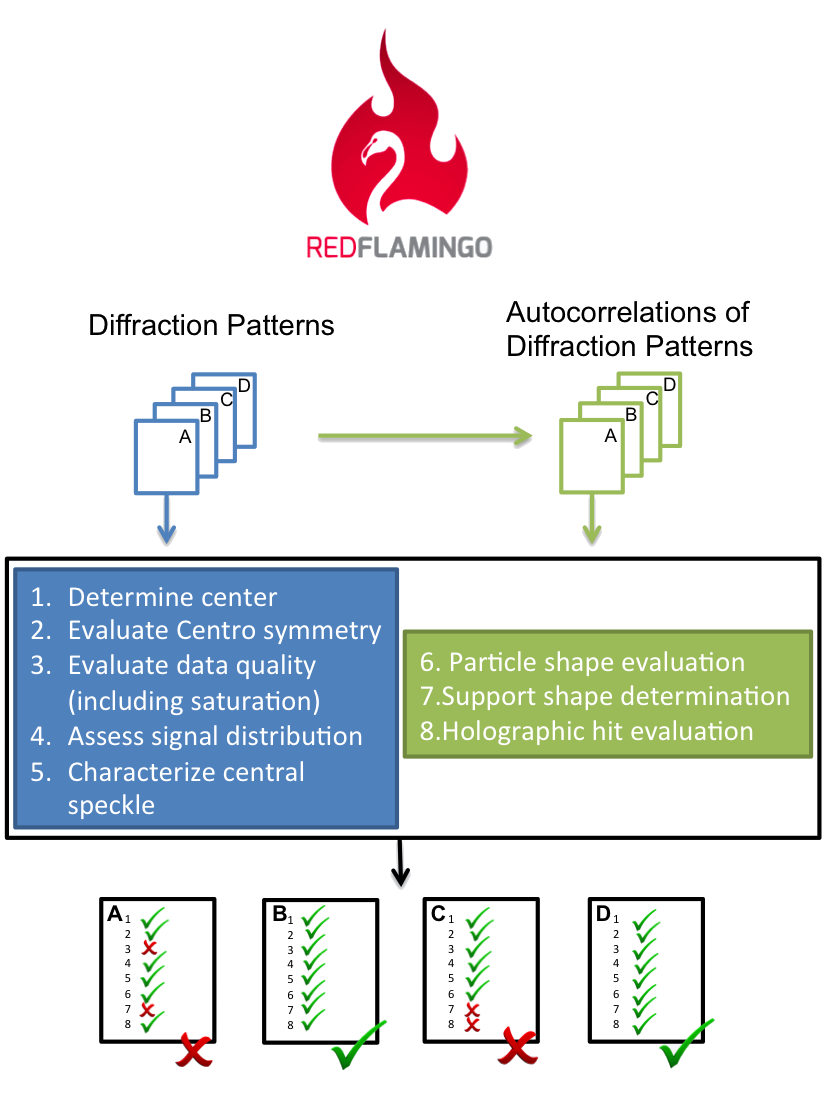
\includegraphics[width=80mm]{Chapter_08_RedFlamingo_Workflow.png}
\caption{The workflow of RedFlamingo. RedFlamingo takes a set of diffraction patterns as input. In this particular workflow eigth different algorithms are selected to assess the diffraction data. Five algorithms evaluate the diffraction patterns themselves, and three are assessing the autocorrelation of the diffraction patterns. As an output RedFlamingo produces a list of scores for each diffraction pattern. Based on the scores, certain patterns can be selected (pattern B and D) or disregarded (pattern A and C). }\label{fig:workflow}
\end{figure}
%\section{Template-based classification}
%If your object has a known shape it could be possible to only select the diffraction patterns that are similar to a set of expected diffraction patterns from the object called templates. Paper III explores the possibility of template-based classification. In general this method is highly dependent on the choice of template, as well as the amount and type of variation present in your sample.

\section{Algorithms implemented in RedFlamingo}
A way of selecting diffraction patterns is by extracting general features from the diffraction pattern such as size, particle shape, amount of saturation, and the number of particles in the beam. Based on the relative values associated with the features, individual patterns can be selected or discarded, or if these values are determined during an experiment, the experimental conditions might be rapidly adjusted. This section describes several feature extraction algorithms I have implemented.

\subsection{Size}
A common method to determine the size of an object is fitting the central speckle to the central speckle of simulated diffraction pattern from a sphere. Such fitting is reliable for particles that themself are close to spherical in shape, such as icosahedrally-shaped viruses (\textbf{Paper XVII},\textbf{Paper XIII}). The second minima is, however, not reliable, as the location of this minima depends on the orientation under which an icosahedron is imaged. If the third to the fifth minima are also present in the diffraction pattern, the average of these minima can also be used reliably to determine the size of the object. This method can be especially useful in case the central speckle or first minimum is affected by saturation effects. Figure \ref{fig:sizing} shows the relative reliability of using different minima to assess the size of an icosahedral object. These results come from simulated diffraction patterns \cite{Hantke2016}.

\begin{figure}[!h]
\centering
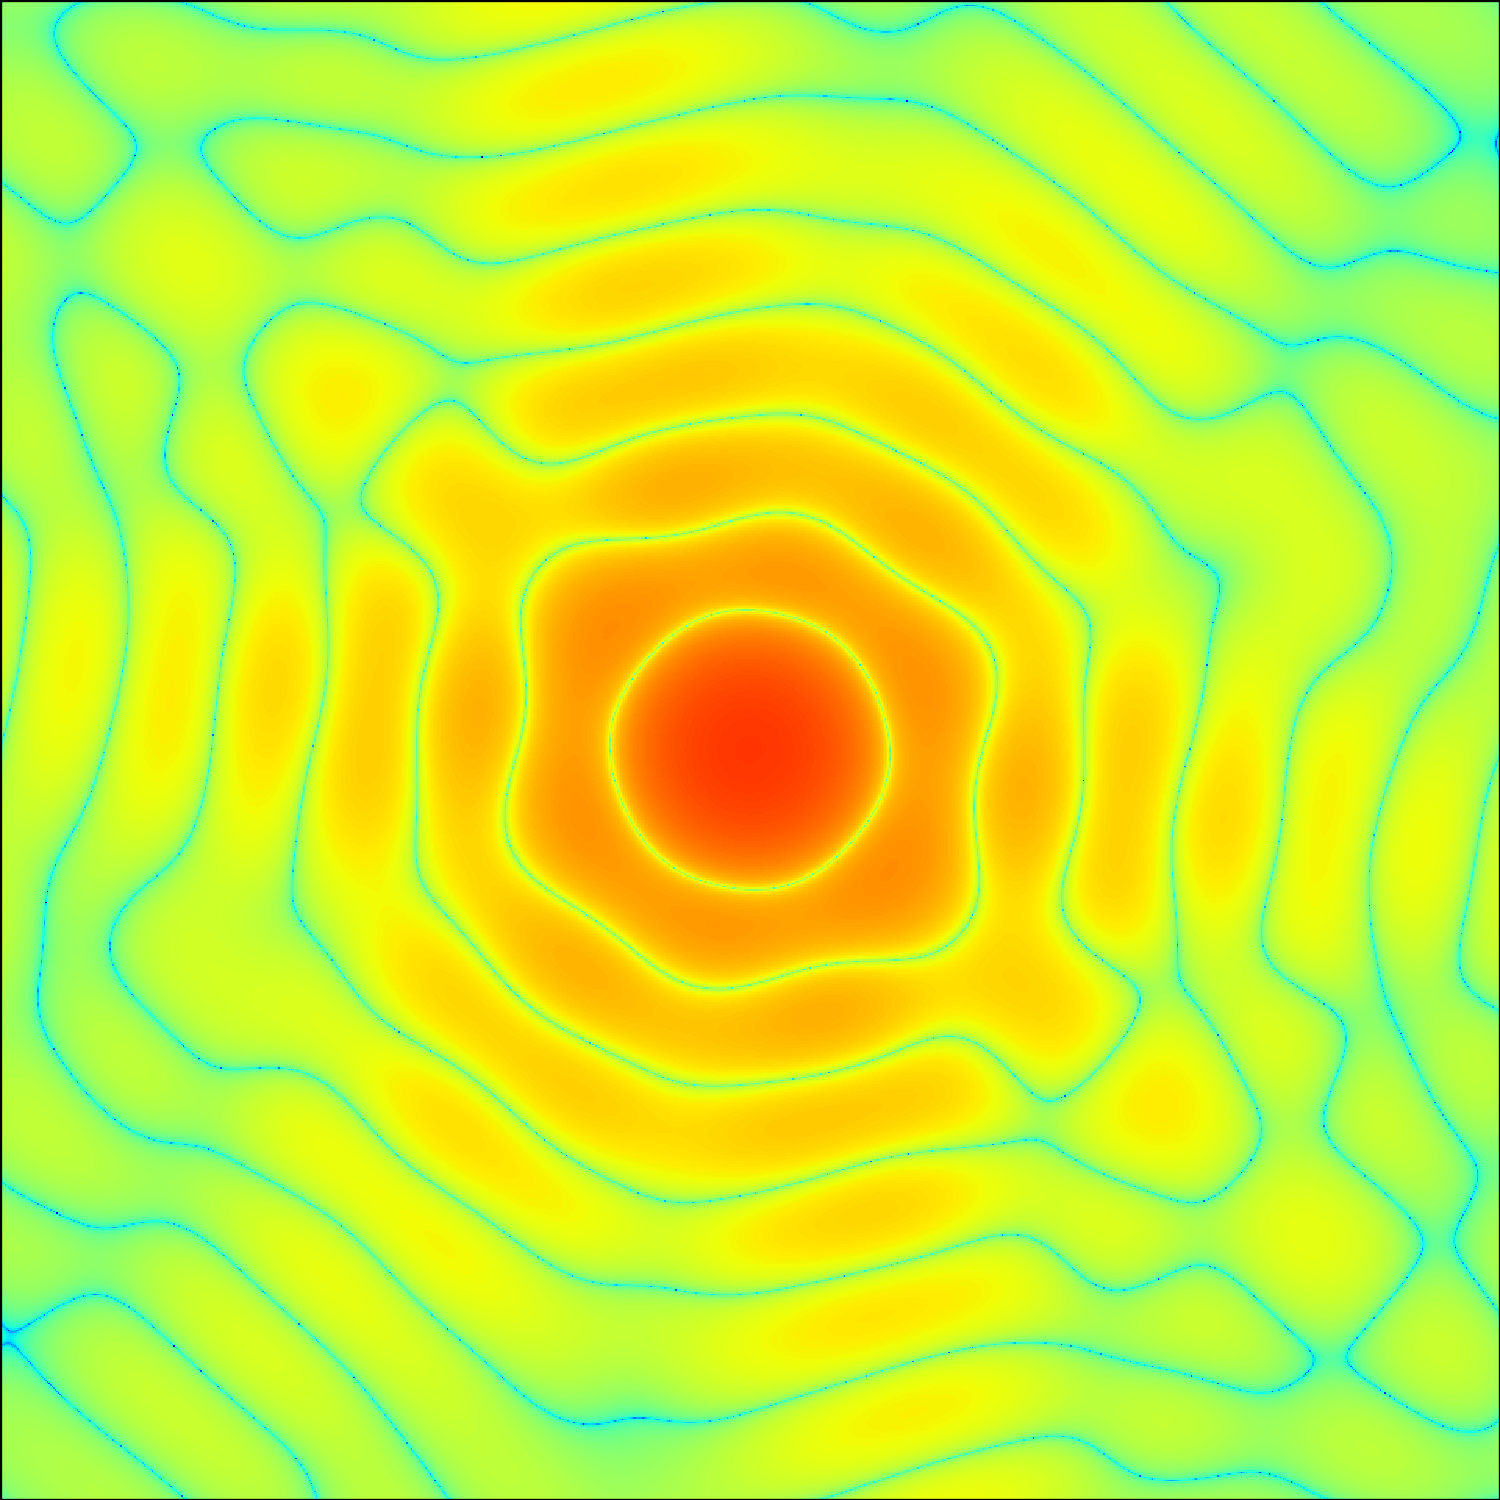
\includegraphics[width=42mm]{Chapter_08_ImageClassification_Simulated_Icosahedron.png}
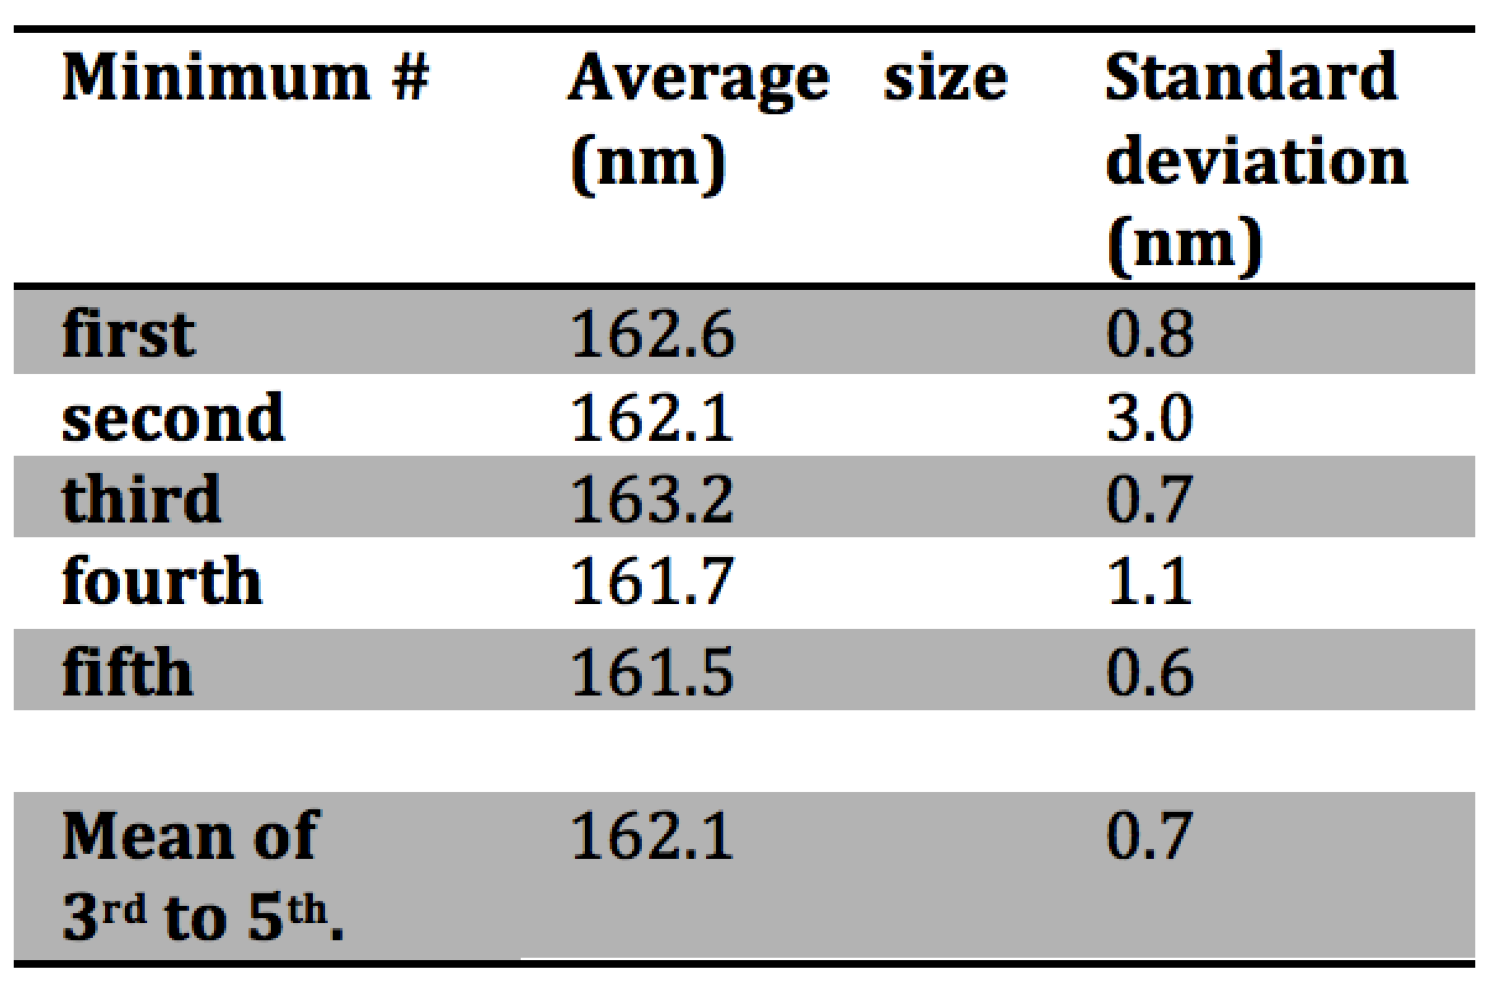
\includegraphics[width=65mm]{Chapter_08_ImageClassification_Stats.png}
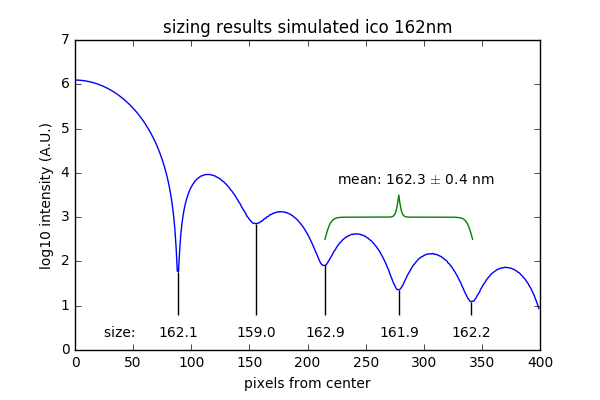
\includegraphics[width=100mm]{Chapter_08_ImageClassification_Sizing_Results.png}

\caption{Evaluation of the size assessment of a icosahedrally shaped particle of 162 nm, using the location of different minima. a) An example of the simulated diffraction patterns used in this evaluation. Each diffraction pattern has a random orientation with respect to the beam. b) The radial average of the diffraction pattern a) with associated size estimates corresponding to the location of each minima. c) the average size estimates based on the location of the each minima, and their respective standard deviations. Although the first minimum is the best in determining the size of an object by itself, the mean of the 3rd - 5th minima are also very good in determining the size of the object.}\label{fig:sizing}
\end{figure}


\subsection{Edge detection / Assess signal distribution radially}
Some objects can be characterized by having sharp edges. A sharp edge in real space corresponds to a streak in the direction perpendicular to the edge in Fourier space. Objects and/or orientations of objects might be classified by determining if, and how many, streaks are present. Figure \ref{fig:edge_detection} explains the idea behind a streak finding algorithm.

\begin{figure}[!h]
\centering
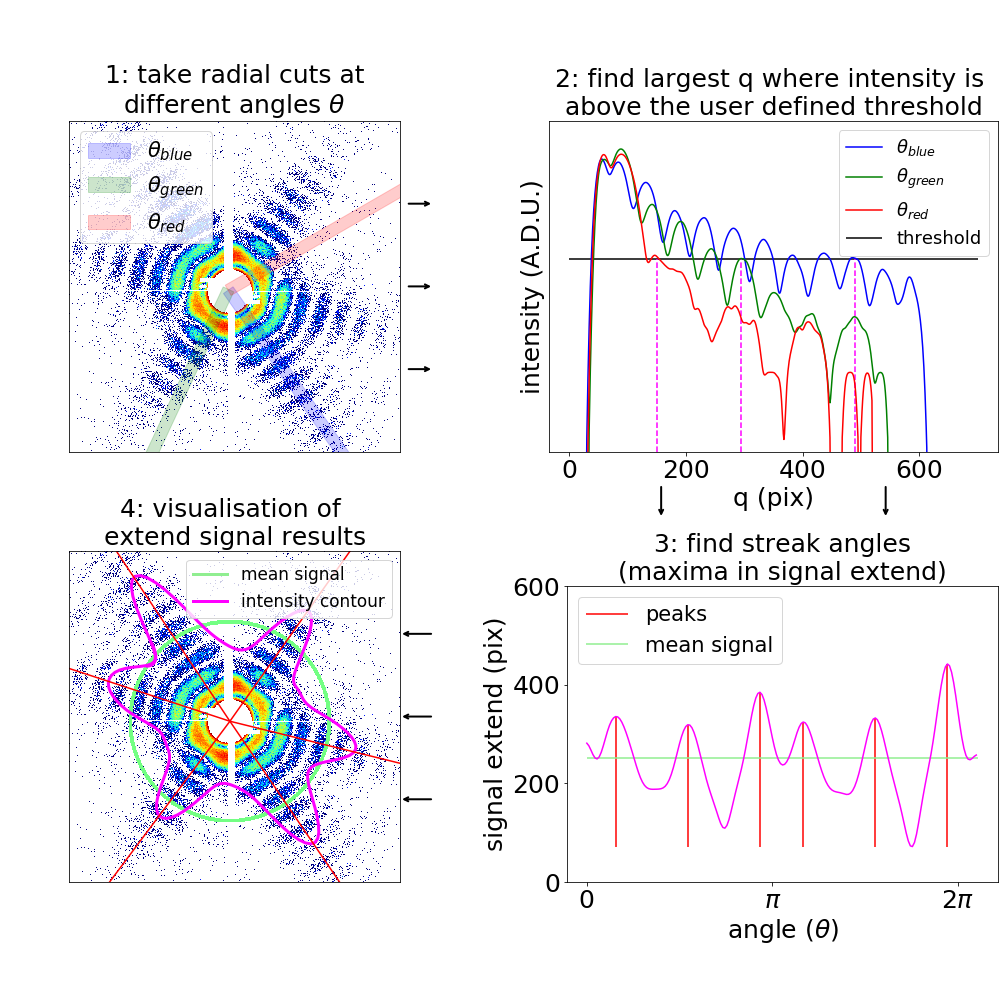
\includegraphics[width=120mm]{Chapter_08_ImageClassification_Edge_Detection.png}
\caption{An evaluation of where in the diffraction pattern the signal is located. In the first step radial cuts are taken each \textit{n} degrees. In 1) only three cuts are visualized: the blue cut is on a streak, the green one is on the edge of a streak, and the red one is in between two streaks. In step 2 the largest distance from the center where the intensity is above a user-defined thereshold is determined. These points are indicated by the dashed magenta lines in 2). The three cuts from 1) show a difference in signal extend. In step three the maxima in the signal extend are determined (see 3). If a maximum has a 180 degree pair, we consider the pair coming from a streak. The average signal extend is indicated by the lightgreen line. 4) The magenta lines contours the signal extend in the diffraction pattern. The red lines indicates the streak location and the lightgreen circle is the mean signal level.}\label{fig:edge_detection}
\end{figure}

\subsection{Elongation}

It might also be possible to determine the elongation of the particle, either by evaluating the elongation of the central speckle (\textbf{Paper XVII},\textbf{Paper XIII}) or by evaluating the elongation of the central term in a filtered autocorrelation. This is useful in discerning between diffraction from spherical and non-spherical objects. Figure \ref{fig:shape_assessment} shows two diffraction patterns: A and B. Diffraction pattern A originates from a icosahedral object and thus has a round central speckle (CS\_A). The fraction of the shortest distance from the center of the central speckle to the edge of the central speckle (minor) divided by the longest distance is called the elongation $\epsilon_{DP}$. Round central speckles have an elongation of 1. The central speckle of pattern B (CS\_B) is much more elongated. 

The evaluation of the autocorrelations of A and B show a similar result. AC\_A shows a roundish particle, whereas AC\_B shows a density that is more elongated. In the radial average of AC\_A and AC\_B this becomes visible as a mass beyond the maximum. The green area is considered to be part of a round particle, and the red area is considered to be part of an elongated particle. The fraction of the green area divided by the green plus the red area constitutes the elongated parameter $\epsilon_{AC}$. The autocorrelation can only be used for the evaluation of convex objects, as non-convex object might appear roundish. 

\begin{figure}[!h]
\centering
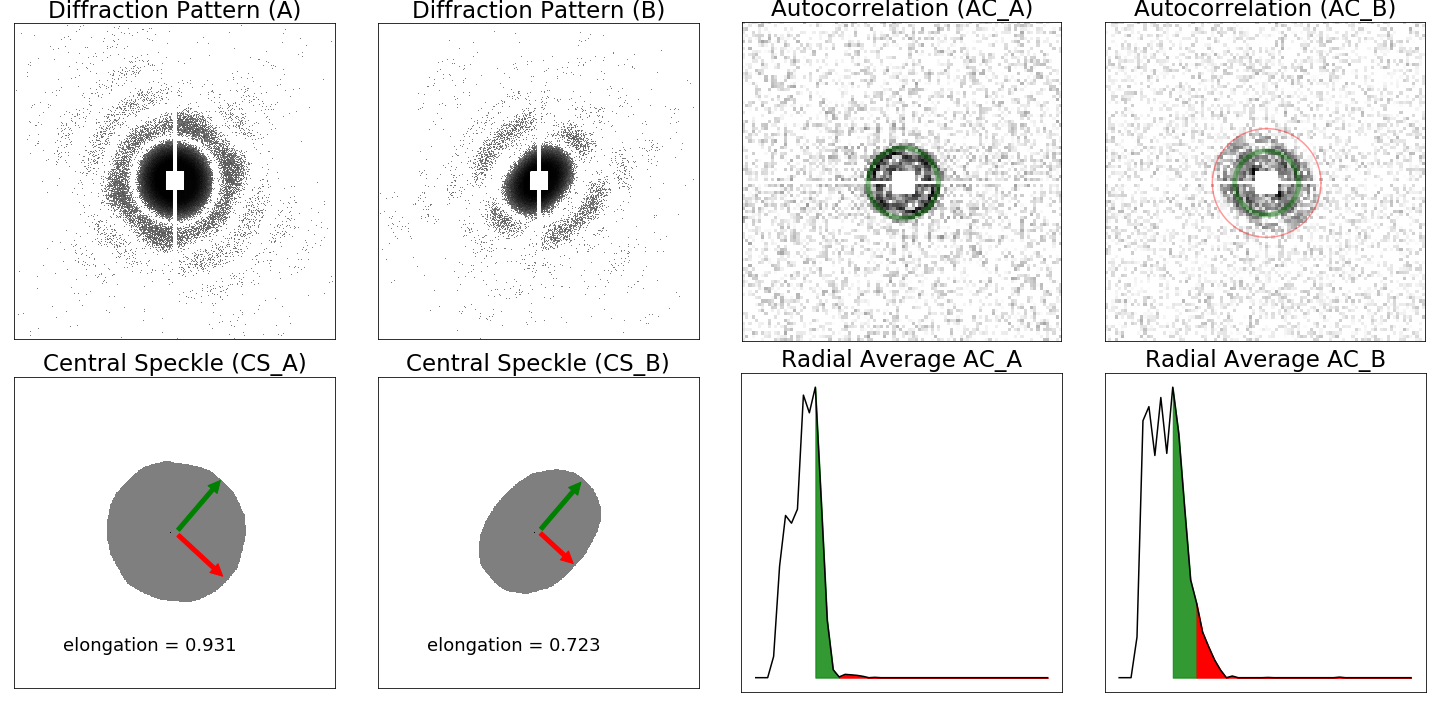
\includegraphics[width=120mm]{Chapter_08_ImageClassification_shape_assessment.png}
\caption{Elongation assessment of the particles that gave rise diffraction pattern A and B. From the central speckles of A and B, CS\_A and CS\_B, have a different shape. The elongation factor $\epsilon_{DP}$ is the fraction of the minor over the major axis of the central speckle. If $\epsilon_{DP}$ is close to 1, the objects that gace rise to the diffraction pattern is considered round in projection. The smaller $\epsilon_{DP}$ the more elongated the particle is considered. The evaluation of the autocorrelation plots show similar results. The central blob in AC\_A is roundish, whereas the central blob is more elongated in AC\_B. In the radial averages of both AC\_A and AC\_B the size of the object is taken as the maximum. The green density is considered part of a spherical object. The red density is considered part of an elongated object. $\epsilon_{AC}$ is the fraction between the green area over the green area + the red area. The closer this fraction is to 1, the more round the particle is considered.}\label{fig:shape_assessment}
\end{figure}


\subsection{The shape of the particle}
An accurate guess for the size of the particle is important for automated phasing. So far automated routines have mainly dealt with icosahedral or round particles, which means the size of the particle, as determined from the central speckle, is enough to determine an accurate support constraint (\textbf{Paper XVII},\textbf{Paper XIII}). The support size and shape of elongated particles such as  cells and many virus species cannot be accurately guessed in this way. Figure \ref{fig:detailed_shape_assessment} illustrates an algorithm that determines the support size and shape of elongated particles by tracing the contour of the central term in a filtered autocorrelation. The algorithm uses Laplace-based edge detection \cite{Mathworks2018}. 

\begin{figure}[!h]
\centering
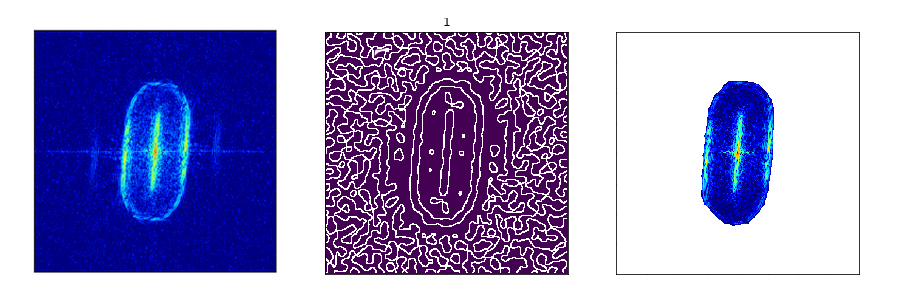
\includegraphics[width=120mm]{Chapter_08_ImageClassification_Refined_Shape_Assessment2.png}
\caption{Finding the shape of the particle. a) shows the filtered autocorrelation of the particle. b) shows the autocorrelation after applying the laplacean edge detection. c) shows the selected area within the autocorrelation. It matches the central term of the autocorrelation. This shape can be used to determining the major and minor size of the particle, and possibly as a guess for the support size and/or shape. }\label{fig:detailed_shape_assessment}
\end{figure}


\subsection{Multiple scatterers in the focus}

Due to the stochastic nature of the injection method, two particles can end up in the interaction region at the same time. If the particles are attached to each other, a similar pattern to the pattern shown in Figure \ref{fig:shape_assessment} will be measured. If the two particles are, however, separated in space, the scattered signal of the two particles will interfere. As a result so called Newton rings will be observed in the diffraction pattern (see Figure \ref{fig:multiplefinding}). As a result of the interference rings, the autocorrelation will show non-central densities, which are called holograms (see \textbf{Paper X}). By determining the presence of non-central terms in the autocorrelation, it is possible to automatically separate the patterns that have interference rings, from patterns that have not. Figure \ref{fig:multiplefinding} illustrates two different methods for finding the non-central density, the first finds the density in the autocorrelation calculated over the entire diffraction pattern. The second method calculates the autocorrelation of a part of the diffraction pattern (similar to a method described in \textbf{Paper XVIII}).

\begin{figure}[!h]
\centering
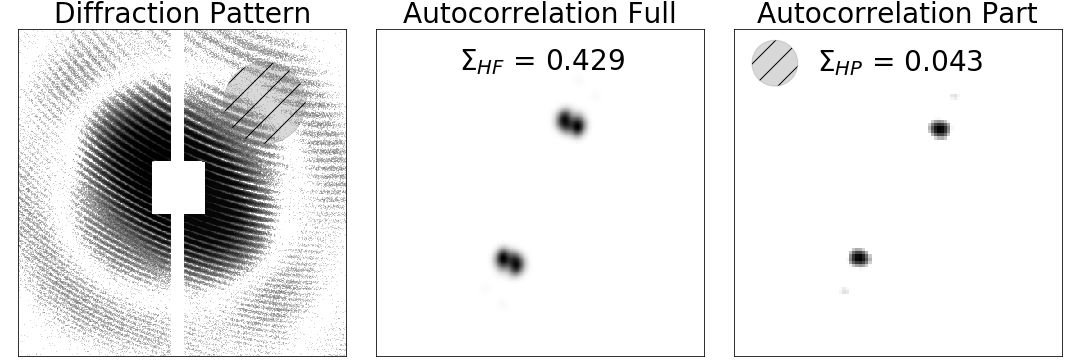
\includegraphics[width=120mm]{Chapter_08_ImageClassification_Multiple_Finding.png}
\caption{Assessing the prescence of multiple particles in the focus, located at a distance from each otherFinding the shape of the particle. a) shows a diffraction pattern which has clear circular interference rings present (center of the rings are somewhere beyond the top left corner. Note the gray circular area. This area of the diffraction pattern is used in c). b) shows the autocorrelation of a) after subtraction an average autocorrelation. The subtraction helps to reduce artefacts coming from the missing data. c) shows the autocorrelation of a small circular area in a). Both methods give two peaks.  }\label{fig:multiplefinding}
\end{figure}